\section{Results}

\subsection{Experimental Setting}
We evaluated our approach on two different datasets and workloads: (1) TPCD-Skew and (2) Conviva.
The TPCD-Skew dataset (1) has the same schema as the TPCD benchmark dataset but sets attribute values drawn from
a Zipfian powerlaw distribution instead of uniformly.
The Zipfian distribution [?] is a long-tailed distribution with a single parameter $z=\{0,1,2,3,4\}$ which a larger
value means a more extreme tail.
The dataset is in the form of a generation program which can generate both the base tables and a set of updates.
For this dataset, we applied our approach to three materialized views, each of a different type:

\vspace{1em}

\textbf{Select-Project View}
\begin{lstlisting}
SELECT *, 
     if(lcase(l_shipinstruct) 
     	     LIKE '%deliver%' 
        AND lcase(l_shipmode) 
             LIKE '%air%',
                  'priority',
                  'slow') 
FROM lineitem_s
\end{lstlisting}

\vspace{1em}

\textbf{Aggregation View}
\begin{lstlisting}
SELECT l_orderkey, 
       l_shipdate, 
       sum(l_quantity) as quantity_sum, 
       sum(l_extendedprice) as extendedprice_sum, 
       max(l_receiptdate) as receiptdate_max, 
       count(*) as group_count 
FROM LINEITEM 
GROUP BY l_orderkey, l_shipdate
\end{lstlisting}

\vspace{1em}

\textbf{Foreign-Key Join View}
\begin{lstlisting}
SELECT supplier.*, 
	   customer.* 
FROM   customer, 
       orders, 
       lineitem, 
       supplier, 
       partsupp 
WHERE  c_custkey = o_custkey 
   AND o_orderkey = l_orderkey 
   AND l_suppkey = ps_suppkey 
   AND l_partkey = ps_partkey 
   AND ps_suppkey = s_suppkey 
   AND s_nationkey <> c_nationkey
\end{lstlisting}

\vspace{1em}

For these three views, we randomly generated aggregation queries and evaluated them for different sample sizes, different update rates, and different parameter settings for the Zipfian distribution.
As a baseline, we evaluate against the following techniques: SAQP, Full Incremental Maintenance, and Recalculation.
In SAQP, rather than estimating a query correction, we incrementally maintain a sample of the view and estimate aggregate queries from only the sample.

\subsection{Query Correction}

\subsubsection{Sample Size and Accuracy}
In this experiment, we illustrate the tradeoff between sample size and accuracy in the TPCD Skew dataset with $z = 2$.
For each of the three views above, we apply the views to a 10GB dataset.
Then, we simulate 5000000 inserted records, corresponding to about 800MB.
We then vary the sampling ratio for the three types of views and show how much sampling is needed to acheive a given query accuracy.
For 10,000 randomly generated aggregation queries on each view, we compare the stale query error to SAQP and our approach.
For SAQP and our approach, we keep the same sampling ratio.
This does, however, mean that SAQP uses significantly more storage than our approach Select-Project and Foreign-Key Join Views.

\begin{figure*}[h]
\label{exp1sample}
\centering
 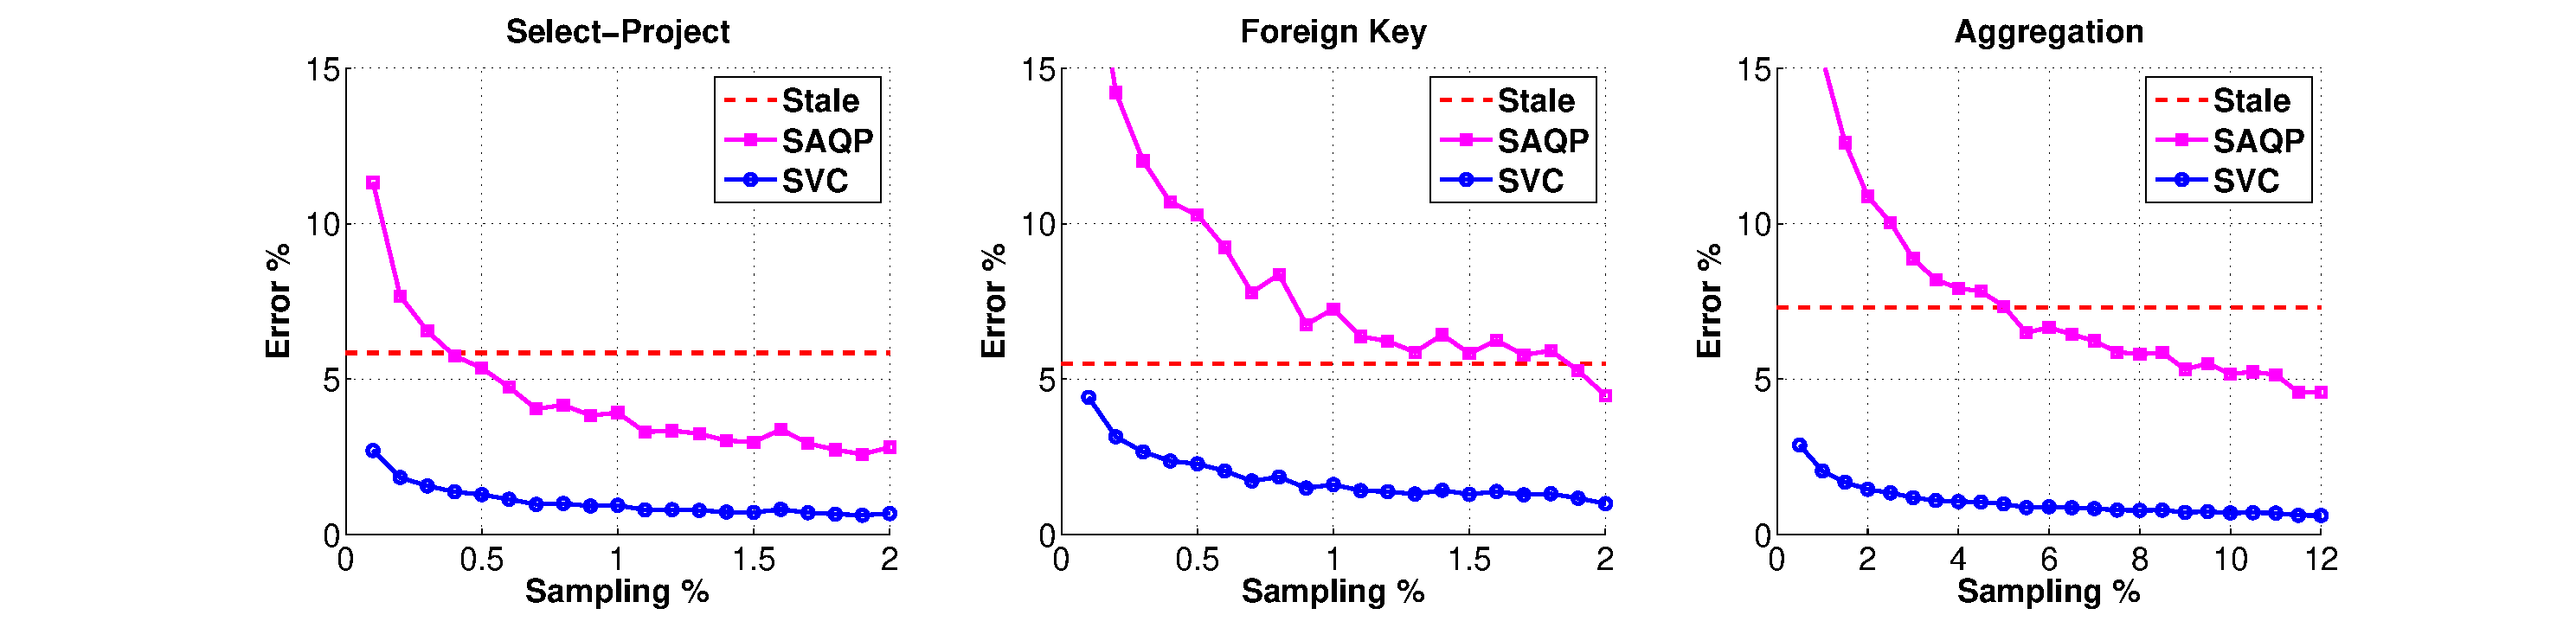
\includegraphics[width=\textwidth]{exp/exp1-samplesize-accuracy.eps}
 \caption{TODO}
\end{figure*}

In Figure \ref{exp1sample}, we show the accuracy as a function of sampling ratio for each of the views.
For both SAQP and our approach, there is a break-even point at which the approximation error is less than the staleness error.
At sampling ratios beyond this point, our query approximated queries are on average more accurate than queries on the stale view.
For all three of the views, the average query error is significantly less than SAQP as the break-even point happens earlier in our approach.

\subsubsection{Update Rate and Accuracy}
In a second experiment, we evaluated the same views and queries but varied the update rate for a fixed sample size.
We set the sample size to $5\%$ and then vary the number of inserted records by increments of 500000 records to a final count of 8000000 records (1.3GB).
Like before, we evalute SAQP and our approach against a baseline stale result.
In Figure \ref{exp2udpate}, we show the results of the experiment. 

\begin{figure*}[h]
\label{exp2update}
\centering
 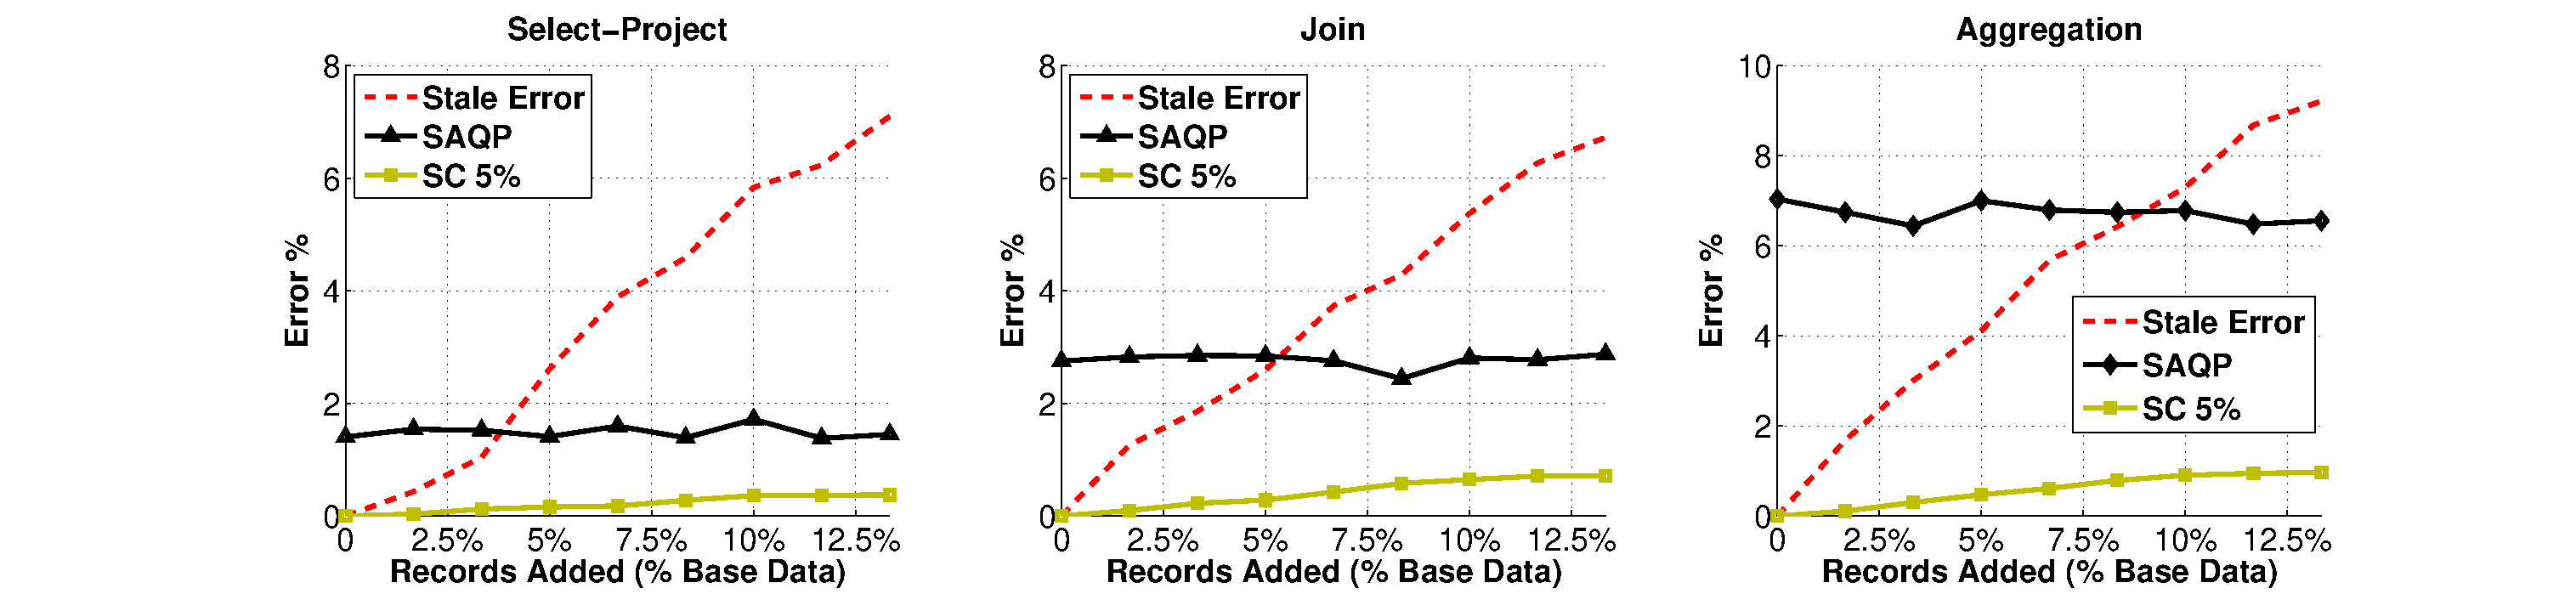
\includegraphics[width=\textwidth]{exp/exp2-updatesize-accuracy.eps}
 \caption{TODO}
\end{figure*}

The results highlight an important point comparing the accuracy of SAQP to our approach. 
The accuracy our approach is proportional to the amount of correction needed, while SAQP keeps a roughly constant accuracy.
As more records are inserted the approximation error in our approache increases.
However, we find that even for very large amounts of inserted records (>10\% of dataset size), our approach gives significantly more accurate results
than SAQP.
The gain is most pronounced in aggregation views where there are a mixture of updated and inserted rows into the view.
Compensationg for a correction to an existing row is often much smaller than doing so for a new inserted record.

\subsubsection{Distribution of Query Error}
In the previous two experiments, we looked at the average error for the queries on the views.
In this experiments, we looked at the distribution of query errors and compared that to their staleness.
For each of the three views, we derive the views from a 10GB dataset.
Then, as before, we simulate 5000000 inserted records and a 5\% sample.
We evaluated the relative error for each query.

\begin{figure*}[h]
\label{exp3dist}
\centering
 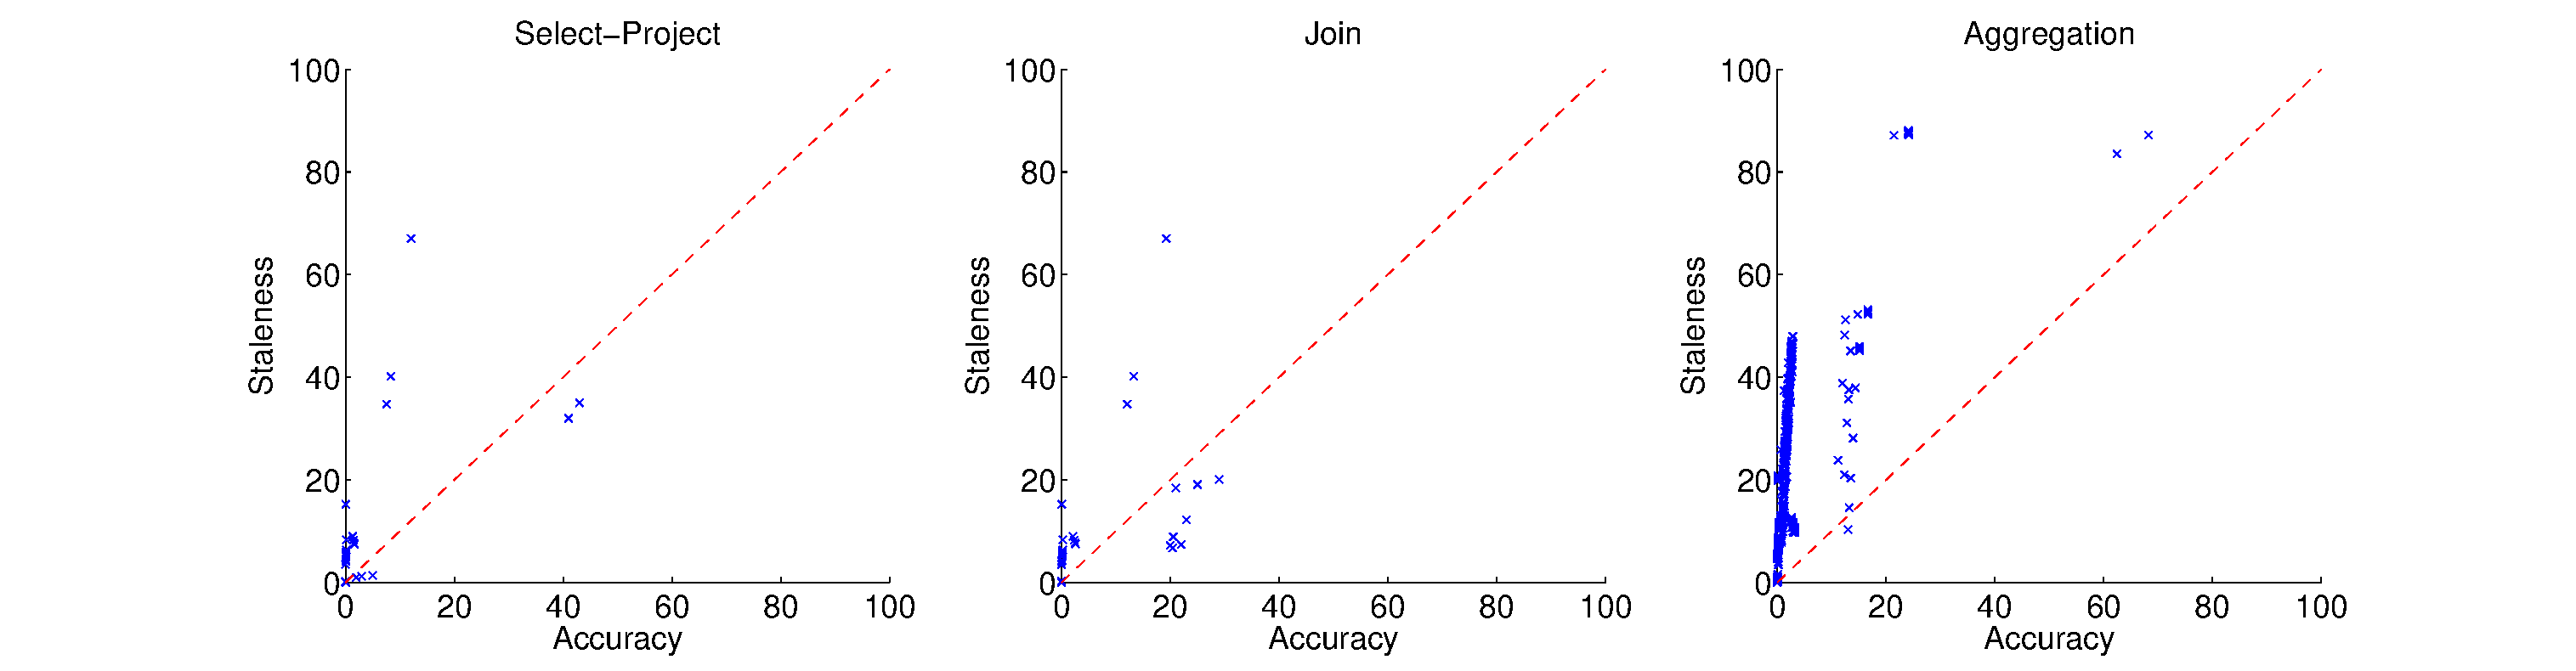
\includegraphics[width=\textwidth]{exp/exp3-query-error-dist.eps}
 \caption{TODO}
\end{figure*}

In Figure \ref{exp3dist}, we present staleness vs. estimation accuracy as a scatter plot.
For all three of the views, the median error is greater than 10 times less than the staleness. 
However, we do see that there are outliers.
Outliers can occur for a variety of reasons.
First, some of the generated queries are highly selective and a uniform sampling approach may not sample enough records to answer it accurately.
Next, outliers can be caused by large updates to the data that are missed by our sampling.
In Section ?, we show how outlier indexing can solve the latter problem and, in fact, after outlier indexing all of our queries on these three views are estimates more accurately than the pre-existing staleness error.

\subsubsection{Computational Efficiency}
We have looked at how small samples can still give highly accurate results.
In this section, we evaluate the efficiency of sampling in terms of computation.
We evaluate our approach on a single r3.large Amazon EC2 node with a MySQL database.
For a batch of updates, we evaluate how long it takes to incrementally maintain a view compared to maintaing a sample.
As before, we derived the views from a 10GB base dataset, and inserted records in increments of 500000.

\begin{figure*}[h]
\label{exp3dist}
\centering
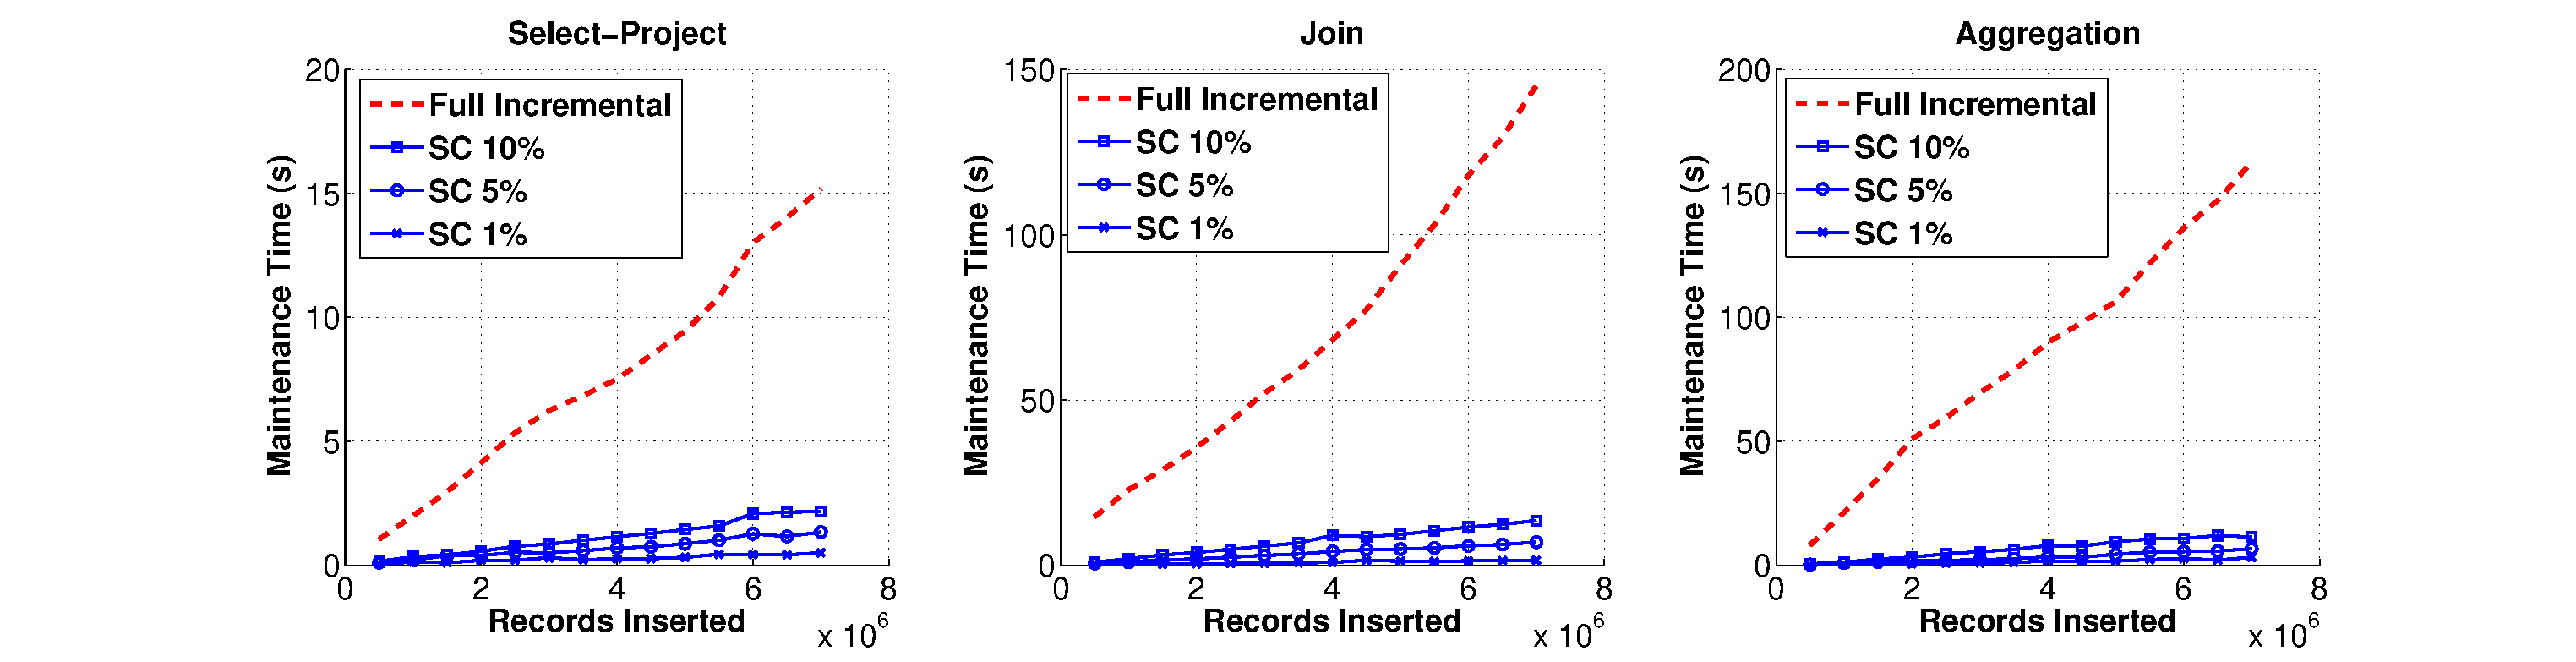
\includegraphics[width=\textwidth]{exp/exp4-efficiency-tpcd-skew.eps}
 \caption{(placeholder) TODO}
\end{figure*}

We find that maintaining a sample is far cheaper than the entire view. In this experiment, keeping a view exactly up-to date required computation on the order of minutes.
However, we found that with a small sample we could acheive this in a few seconds and still acheive accurate results.

\subsection{Outlier Indexing}
TODO

\subsection{Application: Conviva Dataset}
Conviva is a video streaming company that logs activity for each of their videos such as who is watching the video, who owns the video, browser, and network latency etc. 
Analysts from the company answer analytics queries on this dataset such as how many times is a certain video watched.
We experimented with a 1TB dataset of these logs and the corresponding queries on this dataset.
The dataset is a single relation with 103 attributes.
We used the query logs to generate three materialized views.
\vspace{1em}

\textbf{View 1}
\begin{lstlisting}
SELECT clientId, 
       customerId, 
       sessionTimeMs, 
       count(1) 
         as group_count, 
       max(sessionTimeMs) 
         as sessionTimeMs_max, 
       avg(lastBufferLengthMs) 
         as lastBufferLengthMs_avg,
       avg(lLifePausedTimeMs) 
         as lLifePausedTimeMs_avg 
FROM anon_sdm2_ss 
GROUP BY clientId, customerId
\end{lstlisting}

\vspace{1em}

\textbf{View 2}
\begin{lstlisting}
SELECT customerId, 
       sessionType, 
       count(1) as group_count, 
       max(estBwCount) 
           as estBwCount_max, 
       sum(buffTimeMs) 
           as buffTimeMs_sum, 
       sum(estBwCount) 
           as estBwCount_sum 
FROM anon_sdm2_ss 
GROUP BY 
customerId, sessionType
\end{lstlisting}

\vspace{1em}

\textbf{View 3}
\begin{lstlisting}
SELECT justStarted, 
       sessionType, 
       startResourceState, 
       state, 
       count(1) 
            as group_count, 
       max(playTimeMs) 
            as playTimeMs_max, 
       min(stoppedTimeAtJoinMs) 
            as stoppedTimeAtJoinMs_min, 
       max(lifeAverageBitrateKbps) 
            as lifeAverageBitrateKbps_max 
FROM anon_sdm2_ss 
GROUP BY justStarted, 
         sessionType, 
         startResourceState, 
         state
\end{lstlisting}

All three of these views are aggregation views. 
View 1 has the most selective group by clause and was chosen to a be a large view where most of the maintenance is in the form of new rows to insert.
View 2 is a medium size view where maintenance is a mix of both updates and insertions.
View 3 is a small view where most of the maintenance is updates to existing rows.
For these views, we randomly generated aggregation queries.

\subsubsection{Accuracy in Conviva}
We evaluated the average query accuracy for different sample sizes and numbers of records inserted.
Figure \ref{exp5conviva}, compares this accuracy to the staleness of the query.
We find that even a $0.1\%$ sample gives significantly more accurate results for View 1 and View 2.
Even in the situation where the view is small, sampling can still have benefits as seen in View 3.

\begin{figure*}[h]
\label{exp5conviva}
\centering
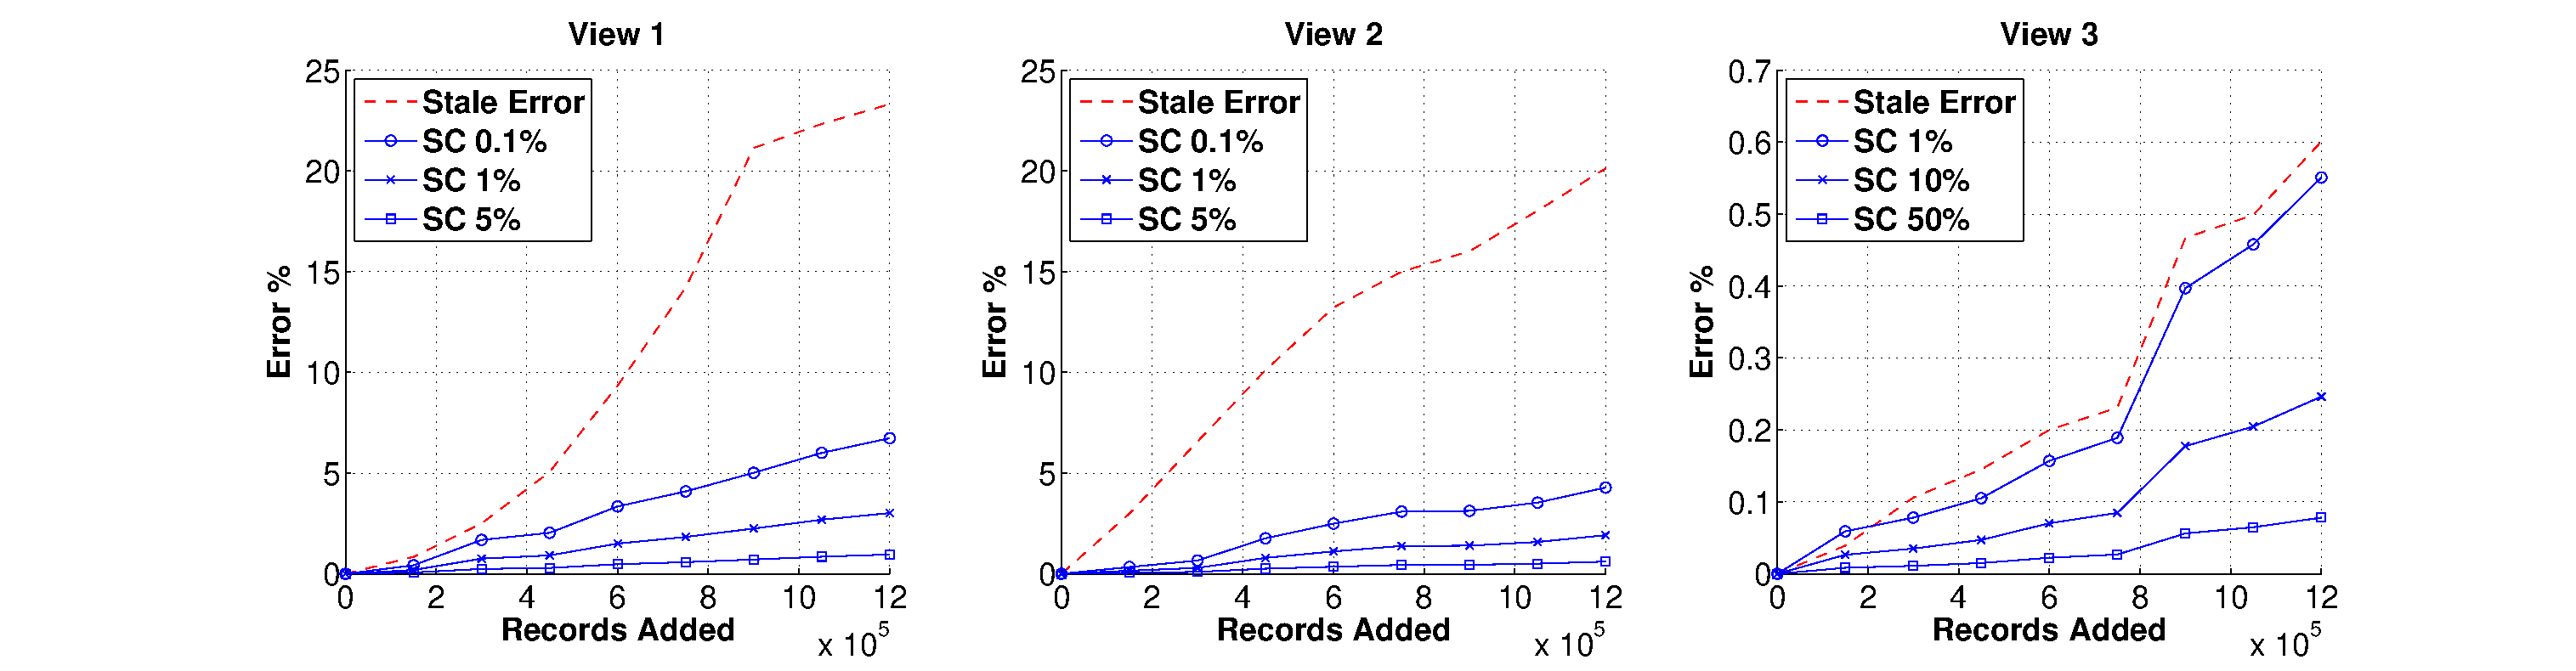
\includegraphics[width=\textwidth]{exp/exp5-coniva-accuracy.eps}
 \caption{TODO}
\end{figure*}

\subsubsection{Performance in Conviva}
We evaluated performance on Apache Spark, on a 20 node r3.large Amazon EC2 cluster. 
This cluster had enough memory to hold all of the materialized views in memory.
Spark supports materialized views through a distributed data structure called an RDD [?].
The RDD's are immutable, thus requiring significant overhead to maintain.
We compare maintenance to recalculation of the view when the data is in memory and when only the updates are in memory. 
We derived the views from a 120GB base relation and inserted records in 10GB increments.

\begin{figure*}[h]
\label{exp6conviva}
\centering
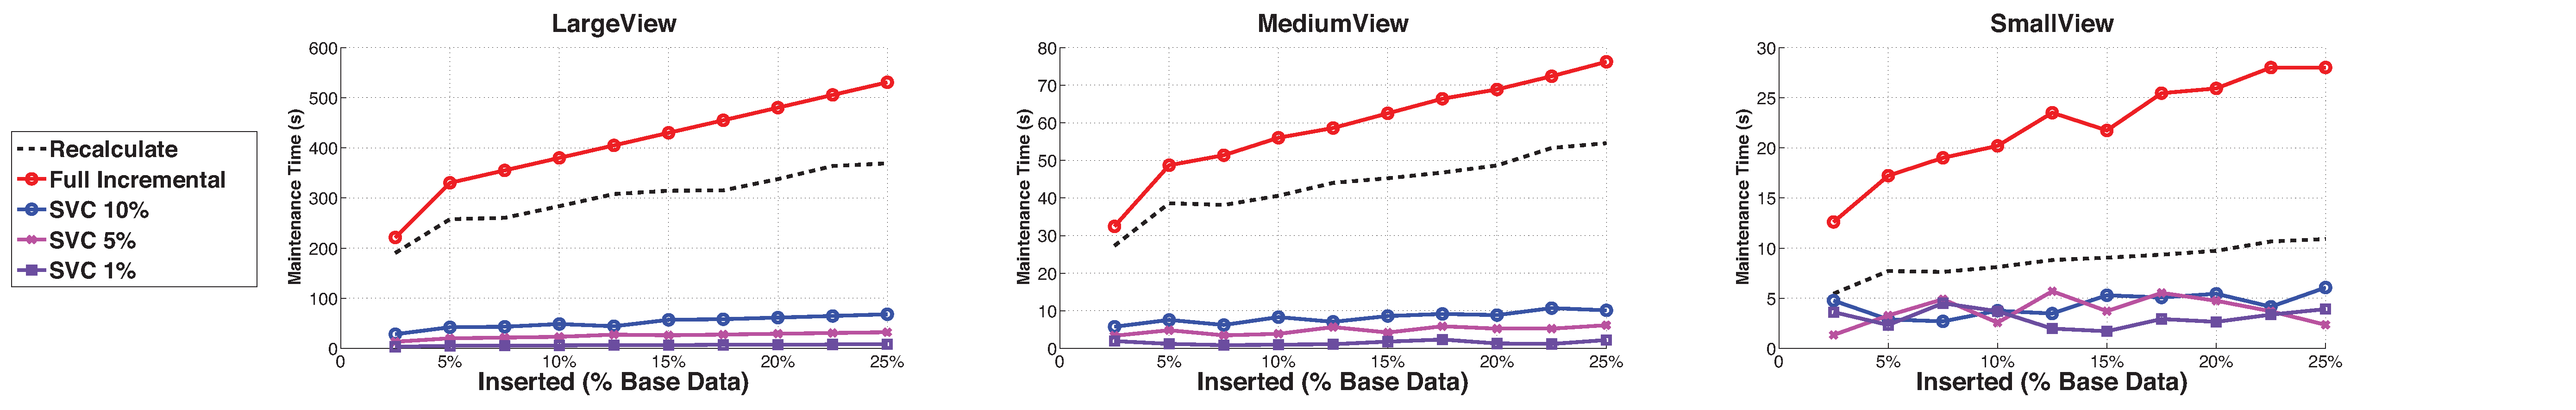
\includegraphics[width=\textwidth]{exp/exp5-efficiency-conviva.eps}
 \caption{(placeholder) TODO}
\end{figure*}

In Figure \ref{exp6conviva}, we illustrate the maintenance time as a function of the number of inserted records.
We find that we acheive good scalability on view 1 and view 2, and still have some performance gains on view 3.
In view 1 and view 2, our gains are more pronounced due to the savings on communication in a distributed environment.
As view 3 is smaller, the communcation gains are less and the only savings are in computation.

